\documentclass[11pt]{article}
\usepackage[a4paper,margin=1in]{geometry}
\usepackage{amsmath,amssymb,booktabs,enumitem,mathtools}
\usepackage[T1]{fontenc}
\usepackage[utf8]{inputenc}
\usepackage{lmodern}
\usepackage{graphicx}
\usepackage{hyperref}

\title{Detailed Note on 5-Fold CV Rank Selection\\for the Matrix Model with $\log_{10}(EC)-\log_{10}(EO)$}
\author{}
\date{\today}

\begin{document}
\maketitle

\section{Purpose}
This note documents the matrix rank-selection procedure implemented in
\texttt{run\_hbn\_trace\_regression\_5fold\_cv\_log\_contrast.py}.
The goal is to select a single matrix rank for the trace regression model when the predictor is restricted to the
\[
\log_{10}(EC)-\log_{10}(EO)
\]
contrast. In this document, ``5-fold CV'' means a single-layer cross-validation procedure:
\begin{itemize}[leftmargin=2em]
    \item the data are partitioned into five folds;
    \item for each candidate rank, the model is fit on four folds and evaluated on the held-out fold;
    \item the final rank is the one with the smallest mean validation MSE across the five folds.
\end{itemize}
There is no inner loop and no nested model selection in this analysis.

\section{Data input and predictor construction}
The input file is
\[
\texttt{hbn\_bandpower\_8band\_roi10.mat},
\]
which contains \(N=397\) subjects. Each subject contributes:
\begin{itemize}[leftmargin=2em]
    \item age as the scalar response \(y_i\);
    \item an \(10\times 8\) eyes-closed (EC) ROI-by-band matrix;
    \item an \(10\times 8\) eyes-open (EO) ROI-by-band matrix.
\end{itemize}
The ten rows correspond to the ROI groups and the eight columns correspond to the canonical frequency bands.

Only one predictor representation is used here. Let \(X_i^{EC}\in\mathbb{R}^{10\times 8}\) and
\(X_i^{EO}\in\mathbb{R}^{10\times 8}\) denote the raw ROI band-power matrices. The analysis first applies the entrywise transform
\[
\widetilde X_i^{EC}=\log_{10}(X_i^{EC}),\qquad
\widetilde X_i^{EO}=\log_{10}(X_i^{EO}),
\]
with a numerical floor
\[
\text{floor}=\max\bigl\{0.5\times \min(\text{positive raw entries}),\,10^{-12}\bigr\}
\]
inserted before taking logarithms. The matrix covariate used in CV is then
\[
X_i=\widetilde X_i^{EC}-\widetilde X_i^{EO}.
\]
Thus the current analysis is a log-contrast analysis, not a relative-power analysis.

\section{Model}
For a candidate rank \(r\), the fitted model is the no-intercept trace regression
\[
y_i=\langle X_i,B\rangle+\varepsilon_i,\qquad \mathrm{rank}(B)\le r.
\]
Here \(B\in\mathbb{R}^{10\times 8}\) is the coefficient matrix and
\[
\langle X_i,B\rangle=\mathrm{tr}(X_i^\top B).
\]

\section{5-fold splitting rule}
The five folds are constructed by a release-stratified split with random seed \(20260320\). The release label is used only for fold construction. For each release,
\begin{itemize}[leftmargin=2em]
    \item the subject indices are shuffled;
    \item the shuffled indices are partitioned into five nearly equal pieces;
    \item the \(k\)-th piece from every release is concatenated to form validation fold \(k\).
\end{itemize}
This preserves release composition across folds up to the discrete partitioning constraint.

\section{Centering within each fold}
Because the model does not include an intercept, centering is carried out inside each training fold.
For fold \(k\), let \(\mathcal I_k^{tr}\) and \(\mathcal I_k^{val}\) denote the training and validation indices. Define
\[
\bar X_k=\frac{1}{|\mathcal I_k^{tr}|}\sum_{i\in\mathcal I_k^{tr}}X_i,\qquad
\bar y_k=\frac{1}{|\mathcal I_k^{tr}|}\sum_{i\in\mathcal I_k^{tr}}y_i.
\]
Then both training and validation data are centered using the \emph{training-fold} means:
\[
X_i^{(k,c)}=X_i-\bar X_k,\qquad
y_i^{(k,c)}=y_i-\bar y_k.
\]
The model is fit on the centered training data, and prediction on the validation fold is performed using the centered validation matrices
\(X_i^{(k,c)}\). Hence the CV comparison is consistent with a no-intercept formulation.

\section{Fixed-rank fitting algorithm}
Given a rank \(r\) and centered training data, the solver minimizes
\[
\min_{\mathrm{rank}(B)\le r}\frac{1}{2n_k}\sum_{i\in\mathcal I_k^{tr}}
\bigl(y_i^{(k,c)}-\langle X_i^{(k,c)},B\rangle\bigr)^2.
\]
The implementation uses projected gradient descent:
\begin{enumerate}[leftmargin=2em]
    \item reshape each matrix \(X_i^{(k,c)}\) into a row of a design matrix \(Z\);
    \item compute a Lipschitz constant
    \[
    L=\sigma_{\max}(Z)^2/n_k;
    \]
    \item set the step size \(\eta=1/L\);
    \item update
    \[
    \widetilde B=B-\eta \nabla f(B);
    \]
    \item project \(\widetilde B\) onto the set \(\{B:\mathrm{rank}(B)\le r\}\) by truncated SVD;
    \item stop when the relative coefficient change or relative objective change drops below \(10^{-7}\), or when
    \(4000\) iterations are reached.
\end{enumerate}
The candidate ranks searched in this run are
\[
r\in\{1,2,\ldots,8\},
\]
because the matrix size is \(10\times 8\).

\section{Validation criterion and rank choice}
For each rank \(r\), fold \(k\), and fitted matrix \(\widehat B_{r,k}\), the validation MSE is
\[
\mathrm{MSE}_{r,k}
=
\frac{1}{|\mathcal I_k^{val}|}
\sum_{i\in\mathcal I_k^{val}}
\bigl(y_i^{(k,c)}-\langle X_i^{(k,c)},\widehat B_{r,k}\rangle\bigr)^2.
\]
The summary criterion is the mean validation MSE
\[
\overline{\mathrm{MSE}}_r=\frac{1}{5}\sum_{k=1}^5 \mathrm{MSE}_{r,k}.
\]
The selected rank is
\[
\widehat r=\arg\min_{r\in\{1,\ldots,8\}}\overline{\mathrm{MSE}}_r.
\]
If two ranks have exactly the same mean validation MSE, the smaller rank is preferred because the summary table is sorted by
\texttt{(mean\_val\_mse, rank)}.

\section{Result of the current run}
The current run produced the following summary:
\begin{itemize}[leftmargin=2em]
    \item selected rank: \(1\);
    \item mean CV MSE at rank \(1\): \(7.590061\);
    \item standard deviation of foldwise validation MSE at rank \(1\): \(0.877828\);
    \item mean CV \(R^2\) at rank \(1\): \(0.267672\).
\end{itemize}
The foldwise validation MSEs at the selected rank are
\[
[6.703889,\ 6.650621,\ 8.094055,\ 8.629773,\ 7.871965].
\]
The foldwise validation \(R^2\) values are
\[
[0.330486,\ 0.318940,\ 0.182993,\ 0.182682,\ 0.323259].
\]
The rank summary over all candidates is given in Table~\ref{tab:rank-summary}.

\begin{table}[!ht]
\centering
\caption{5-fold CV summary for the matrix log-contrast analysis.}
\label{tab:rank-summary}
\begin{tabular}{rrrrr}
\toprule
Rank & Mean val MSE & SD val MSE & Mean val \(R^2\) & Mean iterations \\
\midrule
1 & 7.5901 & 0.8778 & 0.2677 & 1635.8 \\
2 & 8.5531 & 0.8582 & 0.1756 & 3978.8 \\
4 & 9.1332 & 0.9389 & 0.1207 & 4000.0 \\
3 & 9.2244 & 1.0183 & 0.1125 & 4000.0 \\
7 & 9.2612 & 0.9979 & 0.1064 & 4000.0 \\
8 & 9.3533 & 1.0239 & 0.0980 & 4000.0 \\
5 & 9.3893 & 1.0397 & 0.0956 & 4000.0 \\
6 & 9.4784 & 1.0362 & 0.0866 & 4000.0 \\
\bottomrule
\end{tabular}
\end{table}

\paragraph{Remark.}
In Table~\ref{tab:rank-summary}, an average iteration count of \(4000.0\) means that the corresponding rank hit the iteration cap in the
formal run with \texttt{max\_iter=4000}; it should not be interpreted as a proof that the optimizer would never converge under a larger cap.
Additional diagnostic reruns with larger iteration budgets show that higher ranks can indeed converge, but their validation MSE values remain
larger than the rank-\(1\) MSE reported above, so the rank-\(1\) conclusion is unchanged.

Figure~\ref{fig:mse-curve} plots the mean validation MSE by rank using the output generated by the script.

\begin{figure}[!ht]
\centering
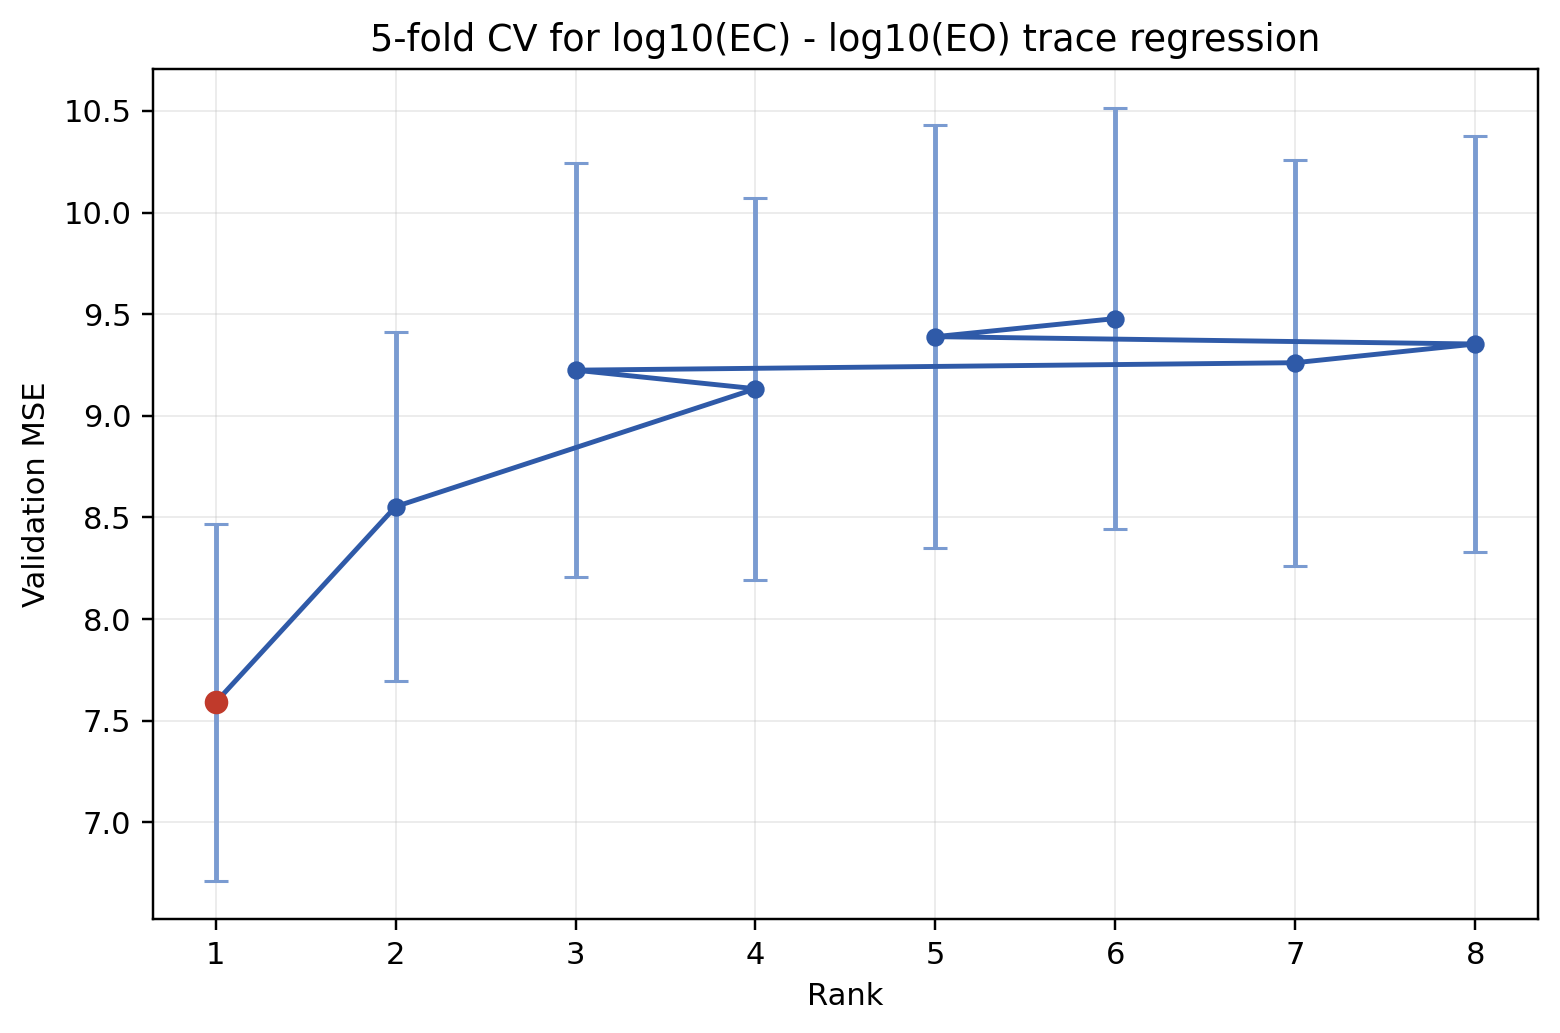
\includegraphics[width=0.72\textwidth]{cv5_mean_mse_by_rank.png}
\caption{Mean validation MSE by rank for the 5-fold CV matrix log-contrast analysis.}
\label{fig:mse-curve}
\end{figure}

\section{Post-selection refit}
After rank selection, the script recenters the full data using the full-sample means and refits the rank-\(1\) model on all subjects.
This step produces
\begin{itemize}[leftmargin=2em]
    \item the selected coefficient matrix \(\widehat B\);
    \item the full-sample centered fitted values;
    \item the coefficient CSV file for downstream interpretation.
\end{itemize}
In the current run, the full-sample centered training MSE at rank \(1\) is \(6.965971\), and the corresponding centered
\(R^2\) is \(0.326381\).

\section{Output files}
The script writes the following files:
\begin{itemize}[leftmargin=2em]
    \item \texttt{cv5\_fold\_manifest.csv}: subject-to-fold assignment;
    \item \texttt{cv5\_rank\_details.csv}: foldwise validation metrics for every candidate rank;
    \item \texttt{cv5\_rank\_summary.csv}: rank-level summary sorted by mean validation MSE;
    \item \texttt{selected\_rank\_1\_coefficients.csv}: fitted coefficient matrix at the selected rank;
    \item \texttt{cv5\_selected\_model.mat}: MATLAB export of the selected model and CV summaries;
    \item \texttt{cv5\_summary.txt}: plain-text summary of the current run;
    \item \texttt{cv5\_mean\_mse\_by\_rank.png}: CV curve used in Figure~\ref{fig:mse-curve}.
\end{itemize}

\section{Interpretation}
Under this single-layer 5-fold CV criterion, the best-performing matrix rank is \(1\). Hence, when the predictor is restricted to
\(\log_{10}(EC)-\log_{10}(EO)\), the data favor the simplest low-rank representation among the searched ranks. In other words,
the validation-error criterion does not support adding extra matrix rank complexity beyond one dominant contrast direction in this setup.

\end{document}
